\chapter{ Identificação de Subsistemas}
\label{sec-subsistemas}

A Figura~\ref{figura-subsistema} mostra os subsistemas identificados no contexto do presente projeto, os quais são descritos na tabela abaixo.




\begin{figure}[h]
  \centering
  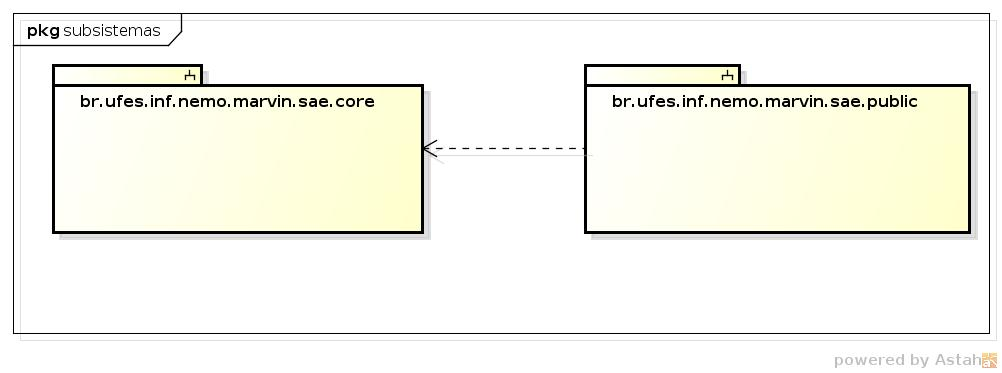
\includegraphics[width=1\textwidth]{figuras/fig-projeto-diagrama-pacotes}
  \caption{Diagrama de Pacotes e os Subsistemas Identificados.}
  \label{figura-subsistema}
\end{figure} 





\begin{table}[h]
	\centering	
	\vspace{0.5cm}
	
	\begin{tabular}{|p{3cm}|p{12cm}|}  \hline \rowcolor[rgb]{0.8,0.8,0.8}
	
 		Subsistema & Descrição \\\hline 
 		                             
		Core & Envolve toda a funcionalidade relacionada com o administrador do sistema, abrangendo controle de Séminarios, Cursos, Assuntos de interesse, envio de email automático e pré-cadastro de egresso. \\\hline
		                              
		Public & Envolve toda a funcionalidade relacionada com consultas a serem realizadas no site, e com as interações que os egressos poderão fazer, tais como cadastrar depoimentos e sugestões. \\\hline 
		
	\end{tabular}
	\caption{ Subsistemas}	
\end{table}
